\chapter{Bibliographic research}
\label{ch:research}

% https://www.ericsson.com/en/reports-and-papers/white-papers/drones-and-networks-ensuring-safe-and-secure-operations
% https://web.stanford.edu/class/cs231a/prev_projects_2016/deep-drone-object__2_.pdf

\section{Remote Drone Control}
\label{sec:research-remote-drone-control}
The article ~\cite{ericsson1} also approaches the topic of drone control. \
According ot it, most current drone use cases cover the situation in which the drone \
operator is in line of sight of the drone and has full control over it, with autonomous \
drones operating outside line of sight gaining more and more importance today. \
However, in the future the most common drone use cases will be the ones in which the drone \
operates autonomously outside line of sight ir without supervision.

\begin{figure}[ht]
    \label{fig:drone-uses}
    %\centering
    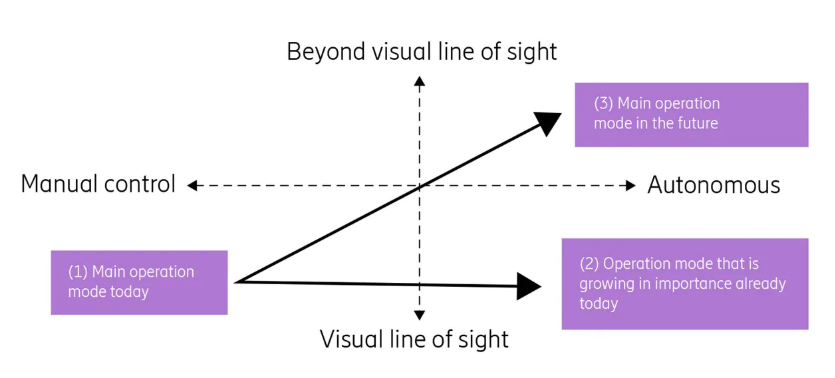
\includegraphics[width=15cm, height=50cm,keepaspectratio]{img/drone_uses.png}
    \caption{Drone Uses according to ~\cite{ericsson1}}
\end{figure}

In ~\cite{ericsson1} mentions three different options for drone communication and control:
\begin{enumerate}
    \item \textbf{satellite technology} is currently in use today for some drones; \
            its drawbacks include high latency and costs and low throughput
    \item \textbf{dedicated drone terrestrial network} its drawbacks also include high \
            costs and the time it would take to setup an adequate coverage for drones
    \item \textbf{existing terrestrial mobile networks} they have low latency and costs and \
            high throughput; \
            additionally, they have also proven to be secure and robust
\end{enumerate}

Additionally, other requirements can be accomplished using 4G LTE and 5G features. \
For instance, drone tracking can be implemented using the mobile positioning service and \
could be queried from the mobile network.

Drone control is also mentioned in ~\cite{forbes1} . \
The article also mentions 2 possible control methods that are actively used and that \
partially overlap over those mentioned above. \
These are:
\begin{enumerate}
    \item \textbf{radio waves} these have limited range (an example of 100 miles is given);
    \item \textbf{satellite uplink} it takes footage an average 1.2-second delay to go from \
            a drone in Afghanistan to the operator in Virginia
\end{enumerate}

~\cite{forbes1} also does a classification of drones according to how they are commanded. \
Three classes of drones emerge:
\begin{enumerate}
    \item \textbf{remotely piloted} an operator has full control, while the drone can do \
            minimal actions by its own, like avoid crashing
    \item \textbf{semi-autonomous} the drone can perform all or some missions without any \
            human interaction, however an operator exists that can take over control at \
            any time
    \item \textbf{fully autonomous} the drone is engineered to accomplish its mission \
            without any human interaction or supervision; \
            the command link can be missing
\end{enumerate}

\section{}


\section{Hyper Heuristics}
\label{sec:research-hh}

\subsection{General Presentation}
\label{subsec:research-general-hh}

In article ~\cite{MetaHeuristicsHandbook}, a hyper heuristic is defined as "\textit{a high-level approach that, \
given a particular problem instance and a number of low-level heuristics, can select and apply an appropriate \
low-level heuristic at each decision point}".\
~\cite{MetaHeuristicsHandbook} also makes several classification of hyper heuristics by several criteria.

\subsubsection{Classification}
\label{subsubsec:research-hh-classification}

Thus, according to ~\cite{soubeiga}, there are 2 types of hyper heuristics:
\begin{enumerate}
    \item \textbf{With Learning} These hyper heuristics make use of a history of low level heuristic efficiency \
and use a learning mechanism to choose some low level heuristics more often than others. Furthermore, this \
cathegory can be split into 2 sub-cathegories, according to the learning mechanism used:
    \begin{enumerate}
        \item \textbf{mechanisms using genetic algorithms}
        \item \textbf{other mechanisms}
    \end{enumerate}
    This distinction can be made because a lot of hyper heuristics have been based at the time of ~\cite{soubeiga} \
on genetic algorithms.
    \item \textbf{Without Learning} There hyper heuristics use multiple low level heuristics, but select them in a \
predefined sequence, no matter their efficiency
\end{enumerate}

~\cite{rbai} and ~\cite{pross} propose a different classification. \
According to them, there are 2 types of hyper heuristics:
\begin{enumerate}
    \item \textbf{Constructive Hyper Heuristics} These hyper heuristics build a solution step by step by selecting \
low level heuristics from a pool at every stage of the construction process.
    \item \textbf{Local Search Hyper Heuristics} These hyper heuristics require a complete solution and select low \
level heuristics to try and improve this solution
\end{enumerate}

According to ~\cite{MetaHeuristicsHandbook}, in the late 2000's a new classification of hyper heuristics emerged, \
inspired by the use of generic programming in the development of hyper heuristics. \
This classification was also mention independently in ~\cite{metabib01} and ~\cite{metabib10}. \
In the new classification, there are also 2 types of hyper heuristics:
\begin{enumerate}
    \item \textbf{"\textit{heuristics to choose heuristics}"} (~\cite{MetaHeuristicsHandbook}) this type of hyper \
heuristics is provided a set of pre-existing, well known low level heuristics for solving a problem, and the hyper \
heuristics select one of these low level heuristics at each step.
    \item \textbf{heuristics to build heuristics} this type of hyper heuristics generate new low level heuristics \
from components or building blocks of known heuristics. It is these newly-built heuristics that will be applied by \
the hyper heuristic.
\end{enumerate}

~\cite{metabib16} presents their own classification of hyper heuristics. \
They identify 4 types:
\begin{enumerate}
    \item hyper heuristics that randomly choose low level heuristics
    \item greedy and peckish hyper heuristics. This type require a pre-run evaluation of the subset of heuristics in \
order to identify the best ones
    \item meta heuristics-based hyper heuristics
    \item hyper heuristics with a learning mechanism used in choosing low level heuristics
\end{enumerate}

~\cite{MetaHeuristicsHandbook} also proposes a new classification, starting from 2 criteria: \textit{the type of \
heuristic search space} and \textit{source of feedback during learning}. \
These criteria can be combined, with different sources of learning being applied to different types of heuristics \
search spaces.

Hyper-heuristics can be grouped into the following categories using the type of heuristic search space:
\begin{enumerate}
    \item \textbf{Selection Hyper-Heuristics} produce groups of already-existing low level heuristics
    \item \textbf{Generation Hyper-Heuristics} produce new low level heuristics using basic building blocks
\end{enumerate}

Using the source of feedback criteria, hyper heuristics can be grouped into the following categories:
\begin{enumerate}
    \item \textbf{Online learning hyper heuristics} learn while solving a problem, similar to unsupervised learning in ml
    \item \textbf{Offline learning hyper heuristics} learn from a set of training data, generating a rule that would \
    apply to other data as well, similar to supervised learning in ml
    \item \textbf{No learning hyper heuristics} no feedback source
\end{enumerate}


%todo: change sub section title
\subsection{Other stuff}
\label{subsec:research-other-stuff}

There are multiple articles that prove the efficiency of hyper heuristics in optimization \
problems, some of which will be presented below. \
Additionally, we will present other methods for generating menus.

In paper ~\cite{ekburke}, a possible hyper heuristic for solving optimization problems in \
planning the scheduling of medical nurses is proposed. \
The purpose of this algorithm wasn't to create an algorithm that is better than other algorithms for this \
specific problem, but to create a method that works well enough, fast enough  and cheap enough for several \
problems and domains. \
Such a method could eventually end up as the basis for multiple cheap \
optimization systems, available to a large number of consumers. \
Additionally, in order to prove the large-scale applicability of of this methods, it was applied to \
university class scheduling. \
The new proposed approach used the same parameters as for scheduling timetable of medical nurses. \
This confirms that the hyper heuristic is not sensitive to parameters when it comes to different types \
of problems, thus having a considerable potential for generalization.




%Bibliographic research has as an objective the establishment of the references for the \
%project, within the project domain/thematic. While writing this chapter (in general the \
%whole document), the author will consider the knowledge accumulated from several \
%dedicated disciplines in the second semester, 4$^{th}$ year (Project Elaboration \
%Methodology, etc.), and other disciplines that are relevant to the project theme.
%
%Represents about 15\% of the paper.
%
%Each reference must be cited within the document text, see example below (depending \
%on the project theme, the presentation of a method/application can vary).
%
%
%This section includes citations for conferences or workshop~\cite{BellucciLZ04}, \
%journals~\cite{AntoniouSBDB07},
%and books~\cite{russell1995artificial}.
%
%In paper~\cite{AntoniouSBDB07} the authors present a detection system for moving obstacles based on stereovision and ego motion estimation.
%The method is ... {\it discus the algorithms, data structures, functionality, specific aspects related to the project theme, etc.}... Discussion: {\it pros and cons}.
%
%In chapter~\ref{ch:analysis} of~\cite{strunk}, the {\it similar-to-my-project-theme algorithm} is presented, with the following features ...
%
%
%\section{Title}
%\section{Other title}
